\documentclass[12pt,openany,a4paper]{book}

%%%%%%%%%%%%%%%%%%%%%%%%%%%%%%%%%%%%%%%%%%
%% Packages
%%%%%%%%%%%%%%%%%%%%%%%%%%%%%%%%%%%%%%%%%%
\usepackage[style=ieee]{biblatex}

\usepackage{geometry}
\usepackage[hidelinks]{hyperref}
\usepackage{nameref}
\usepackage[parfill]{parskip}
\usepackage{listings}


\usepackage{algorithmicx}
\usepackage{algpseudocode}
\usepackage{minted}
\setminted{tabsize=4}

\usepackage{graphics}

\usepackage{titling}
\usepackage{titlesec}

%\usepackage{showframe}

%%%%%%%%%%%%%%%%%%%%%%%%%%%%%%%%%%%%%%%%%%
%% Settings
%%%%%%%%%%%%%%%%%%%%%%%%%%%%%%%%%%%%%%%%%%

\titlespacing*{\subsubsection}
{0pt}{\baselineskip}{0.5\baselineskip}

%%%%%%%%%%%%%%%%%%%%%%%%%%%%%%%%%%%%%%%%%%
%% Macros
%%%%%%%%%%%%%%%%%%%%%%%%%%%%%%%%%%%%%%%%%%

\newcommand{\mono}[1]{\texttt{#1}}

\newcommand{\monotuple}[1]{$ \left\langle \right. $\mono{#1}$ \left. \right\rangle $}

% JIF
\newcommand{\jiflabel}[1]{\mono{\{#1\}}}

% Paragon
\newcommand{\paralabel}[2]{\jiflabel{#1:$ \; $#2}}
\newcommand{\generic}[1]{$ < $#1$ > $}

%%%%%%%%%%%%%%%%%%%%%%%%%%%%%%%%%%%%%%%%%%
%% Document
%%%%%%%%%%%%%%%%%%%%%%%%%%%%%%%%%%%%%%%%%%

\title{The Applicability of Information Flow to Secure Java Development}

\bibliography{content/bib/bibliography}

\begin{document}
	
	\frontmatter
	
	% A titlepage template found online by David Buchan-Swanson a long time ago, and modified to fit the uses required.  If you own this, please contact me.

\begin{titlepage}

\newcommand{\HRule}{\rule{\linewidth}{0.5mm}} % Defines a new command for the horizontal lines, change thickness here

\centering % Center everything on the page
 
%----------------------------------------------------------------------------------------
%	HEADING SECTIONS
%----------------------------------------------------------------------------------------

\textsc{\LARGE The University of Queensland}\\[1cm] % Name of your university/college
\textsc{\Large ENGG4801 -- Thesis}\\[0.5cm] % Major heading such as course name

%----------------------------------------------------------------------------------------
%	TITLE SECTION
%----------------------------------------------------------------------------------------

\HRule \\[0.4cm]
{ \huge \bfseries Project Proposal}\\[0.2cm]
{\huge Analysis of the Security Properties of Java Programs}
\HRule \\[.5cm]
 
%----------------------------------------------------------------------------------------
%	AUTHOR SECTION
%----------------------------------------------------------------------------------------

\begin{minipage}{0.45\textwidth}
\begin{flushleft} \large
\emph{Author:}\\
Joseph Spearritt | 43590441
\end{flushleft}
\end{minipage}
~
\begin{minipage}{0.45\textwidth}
\begin{flushright} \large
\emph{Supervisors:}\\
Dr Larissa Meinicke\\
Professor Ian Hayes
\end{flushright}
\end{minipage}\\[1.5cm]

% If you don't want a supervisor, uncomment the two lines below and remove the section above
%\Large \emph{Author:}\\
%John \textsc{Smith}\\[3cm] % Your name
%\begin{minipage}{0.45\textwidth}
%\begin{flushleft}\large
%\emph{Lecturer:} \\
%Professor Penelope \textsc{Sanderson}\\
%[.5cm]
%\end{flushleft}
%\end{minipage}\\[.7cm]

%----------------------------------------------------------------------------------------
%	DATE SECTION
%----------------------------------------------------------------------------------------

%{\large \today}\\[.5cm] % Date, change the \today to a set date if you want to be precise

%----------------------------------------------------------------------------------------
%	LOGO SECTION
%----------------------------------------------------------------------------------------

%\includegraphics[width=.4\linewidth]{logo.png}\\[.5cm] % Include a department/university logo - this will require the graphicx package


\end{titlepage}
	
\cleardoublepage

\begin{flushright}
	ADDRESS LINE 1\\
	ADDRESS LINE 2\\
	Tel.\ (07) nnnn nnnn\\
	\medskip
	\today
\end{flushright}
\begin{flushleft}
	Prof Paul Strooper\\
	Head of School\\
	School of Information Technology and Electrical Engineering\\
	The University of Queensland\\
	St Lucia, Q 4072\\
	\bigskip\bigskip
	Dear Professor Strooper,
\end{flushleft}

In accordance with the requirements of the degree of Bachelor of Engineering in the division of Software Engineering, I present the following thesis entitled ``\thetitle''. This work was performed under the supervision of Dr Larissa Meinicke \& Prof Ian Hayes.

I declare that the work submitted in this thesis is my own, except as
acknowledged in the text and footnotes, and has not been previously
submitted for a degree at The University of Queensland or any other
institution.

\begin{flushright}
	Yours sincerely,\\
	\medskip
%	\emph{Author's Signature}
	$ \; $\vspace*{5mm}\\
	\medskip
	Joseph Spearritt.
\end{flushright}

\cleardoublepage

\chapter{Acknowledgements}

Acknowledge your supervisor, preferably with a few short and specific
statements about his/her contribution to the content and direction of
the project.  If you collaborated with another student, acknowledge
your partner's contribution, including any parts of the thesis of
which s/he was the principal author or co-author; this information can
be duplicated in footnotes to the chapters or sections to which your
partner has contributed.  Briefly describe any assistance that you
received from technical or administrative staff.  Support of family
and friends may also be acknowledged, but avoid sentimentality---or
hide it in the dedication.

\chapter{Abstract}

Some abstract stuff goes here
	
	\tableofcontents
	
	\listoffigures
	
	\listoflistings
	
%	\listoftables
	
	\mainmatter
	
	\section{Introduction}

\begin{frame}{Java is Widely Used}
	As one of the most widely used languages on the planet, a lot of security critical code is written in Java.
	
	Due to its prevalence on the desktop, mobile and (formerly) the web, developers depend on the security of the JRE, of libraries, and of their trusted code.
	
	If any one of those components has a vulnerability, the system may be compromised.
\end{frame}

\begin{frame}{Java is Vulnerable}
	\begin{columns}
		\column{0.55\textwidth}
			37 vulnerabilities were recorded in the US National Vulnerability Database in 2016.\newline
			
			13 were listed as `critical', with a CVSS score $ > $ 9.0, indicating complete compromise of Confidentiality and Integrity \cite{nvd:jdk2016cvss9}.
		\column{0.45\textwidth}
		\begin{figure}
			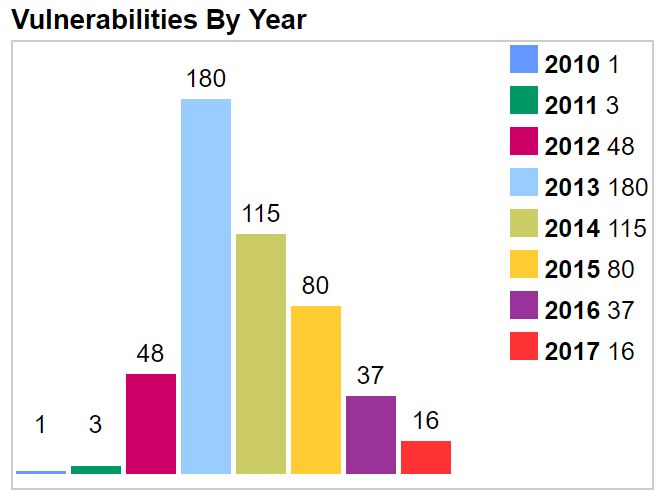
\includegraphics[scale=0.25]{content/images/cvedetails_vulnsperyear.png}
			\caption{Total CVEs by year \cite{cvedetails:jdk2016}}
		\end{figure}
	\end{columns}	
\end{frame}

\begin{frame}{Writing Secure Java Code}
	Developers of security conscious Java applications must ensure the Confidentiality, Integrity and Availability of data. They can do this by:
	
	\begin{itemize}
		\item Following the Oracle Secure Coding Guidelines
		\item Running their application with a \texttt{SecurityManager} installed
		\item Following the Principle of Least Privilege
	\end{itemize}
	
	What they usually can't do is \textit{prove it}.
\end{frame}

\begin{frame}{Thesis Topic}
	One avenue for providing \textit{provable} Confidentiality and Integrity to programs is applying the theory of \textit{Information Flow}, leading to the key question:
	
	\begin{block}{Key Thesis Question}
		Can Information Flow be used to provide practical improvements to the Confidentiality and Integrity of Java programs?
	\end{block}
	
	To answer this question, this thesis aims to evaluate both the relevance of information flow-based security, and current implementations of it, to determine:
	
	\begin{enumerate}
		\item What practical security benefits Information Flow can provide
		\item Whether Information Flow is viable for real world applications
	\end{enumerate}
\end{frame}
	
	\chapter{Background \& Theory} \label{chap_theory}

\section{Security Context}

Information security in practice revolves around three key goals colloquially known as the `CIA Triad' \cite{krutz2010cloudsec}:

\begin{itemize}
	\item Ensuring information is appropriately \textit{Confidential}

	\begin{itemize}
		\item Example: a secret password being leaked is a confidentiality violation
	\end{itemize}
	
	\item Ensuring information has \textit{Integrity}
	
	\begin{itemize}
		\item Example: a database being accessed and records falsified is an integrity violation
	\end{itemize}
	
	\item Ensuring information is \textit{Available}
	
	\begin{itemize}
		\item Example: a Denial of Service (DoS) attack causing a website to crash is an availability violation
	\end{itemize}

\end{itemize}

Most language-based security features focus on the confidentiality and integrity of information; that is, ensuring that secret information remains secret, and that information which needs to be trusted is, in fact, trustworthy.

The most common mechanism used in computer systems to ensure confidentiality and integrity is \textit{access control}: associating some `permissions' with users of a system and restricting the actions they are able to perform based on these permissions.

\section{The Java Security Model}

The Java programming language was designed in the context of emerging internet technologies, with the explict use case of users downloading and running `applets' from web pages. As such, security was a core consideration of Java's design -- the original design goals document \cite{javadesignprinciples} specifies that ``applications written in the Java programming language are secure from intrusion by unauthorized code."

Java is type safe and memory safe, which reduces the possibility of programmer error leading to exploitable flaws in an application. Java's application sandbox takes a three-pronged approach to security in the context of applets which may be downloaded from a remote server, with the Bytecode Verifier, the Class Loader, and the Security Manager \cite{mcgraw1999securingjava}.

The Bytecode Verifier and the Class Loader concern the loading of new classes into a running Java Virtual Machine (JVM). The Bytecode Verifier analyses the class to ensure it maintains the class format, does not perform illegal casts, and that it obeys Java's typing rules more generally (e.g. that private methods may not be accessed outside of a class, final methods may not be overridden) \cite{lindholm2014java}. The Class Loader performs the actual loading of a class into the JVM; the `primordial' Class Loader \cite{mcgraw1999securingjava} loads the Java API classes, and other classes may be loaded by a user-specified \mono{ClassLoader} instance.

\subsection{The Security Manager \& Stack Inspection}

The final element of the sandbox model is the \mono{SecurityManager} class. When enabled, an instance of \mono{SecurityManager} runs in the JVM, and performs runtime access control: when a potentially sensitive action is undertaken, the Security Manager checks the permissions of the calling class based on the system policy (usually specified by an external policy file), and throws an exception if the permission check fails \cite{gosling2014java}.

Permission checks are performed using stack inspection \cite{gong2003javasecurity}: every frame on the call stack below the sensitive operation is examined, and if \textit{any} frame does not have the required permissions, the check fails. Java provides the \mono{doPrivileged} construct to bypass full stack inspection \cite{gong2003javasecurity} where this is desired functionality.

\section{Information Flow Security}

Access control mechanisms limit the \textit{permissions} of a subject attempting to access data. Many programs and operating systems make use of \textit{Discretionary} Access Control, which models permission via Access Control Lists specifying what items individual users or groups of users may access (for example: the Unix permissions system). What such mechanisms cannot restrict is the way in which information \textit{propagates}.

Under Discretionary Access Control, only authorised users may access a piece of data. But once access is given, there are no controls on what the user may do with it. \textit{Information Flow} mechanisms seek to improve this, by enforcing some policy on the data itself, so even if a user may \textit{access} the data, there are restrictions on how they may propagate that data.

\section{Mandatory Access Control \& The Lattice Model}

The most well-known model designed to deal with Information Flow security, Mandatory Access Control (MAC), is most commonly associated with the military and other high-security organisations. In a MAC system, all data has a \textit{classification}, and users operate with a \textit{clearance}. 

In the simplest case, the set of classifications is just an ordered list -- for instance, `Unclassified' $ < $ `Classified' $ < $ `Secret' $ < $ `Top Secret'. A user with `Secret' clearance, then, cannot access or modify `Top Secret' documents.

More flexible access control policies may be implemented under the Bell-Lapadula lattice model \cite{bell1973lattice}, which is at the heart of most modern MAC systems. Under this model, classifications form a \textit{lattice} -- a set partially ordered by a flow relation (written $ \succeq $) where, for every possible pair of elements, a `least upper bound' (or `join', written $ \sqcup $) and `greatest lower bound' (or `meet', written $ \sqcap $) may be found.

In the MAC context, for policies in a lattice structure it is always possible to determine whether a user at clearance $ A $ can access information at classification $ B $ -- they can if $ B \succeq A $. Given any two classifications $ A $ and $ B $, one can find the least restrictive classification which enforces both, $ A \sqcup B $, and the most restrictive classification which users at either clearance $ A $ or $ B $ can read, $ A \sqcap B $.

MAC is applied to the an access control problem concerning users (or `subjects') and classified documents (or `objects') via two key rules \cite{sandhu1993lattice}:

\begin{description}
	\item[Simple Security Property -- `No Read Up'] A subject with clearance $ C_s $ may access an object with classification $ C_o $ if and only if $ C_s \succeq C_o $
	
	\item[* Property -- `No Write Down'] A subject with clearance $ C_s $ may only modify an object with classification $ C_o $ if $ C_o \succeq C_s $
\end{description}

The Simple Security Property prevents users with insufficient clearance from accessing highly classified data. But the * Property is also important: it states that a user with high clearance cannot modify data at a low classification. This prevents a highly privileged user from declassifying data by copying it to a document with lower classification, thereby introducing a control on the \textit{propagation} of that information.

Lattice-based Mandatory Access Control may be applied to computer systems, just as to physical documents. Such systems generally use a `high water mark' approach \cite{jones1975highwatermark}, allowing programs to begin at low clearance and only moving to higher clearance as needed.

\section{Formal Non-interference}

The traditional MAC model may be implemented in a real system via runtime-enforced access control checks. However, the fundamental question remains: how does the program's author know whether it's implemented \textit{correctly}? Many security issues are the result of unintentional programmer error, and so it is useful to approach Information Flow security from the perspective of program verification.

This goal can be more clearly defined through the notion of `non-interference'. A program is said to be non-interfering if, given any two program executions which are identical in terms of their low confidentiality input, the results and behaviour of the executions are indistinguishable \cite{sabelfeld2003if}. If a program is non-interfering with respect to a MAC policy, then by definition it correctly follows that policy. This notion may be formalised by the definition that a program is non-interfering if there is no \textit{dependency} of low confidentiality data on high confidentiality data \cite{cohen1977declassification}.

In \citetitle{denning1977certification}, \citeauthor{denning1977certification} \cite{denning1977certification} provide a mechanism which can verify a program as correctly respecting a MAC policy using type-checking: all variables are assigned a classification, and the analyser ensures that the policy is not broken under any execution path.

\subsection{Implicit Flows}

For a program to be non-interfering, a passive attacker must not be able to distinguish \textit{any} information about high confidentiality data. It is not sufficient to simply prevent a high confidentiality value from being assigned to a low confidentiality variable -- for instance, consider the following case:

\begin{algorithmic}
	\State $ high := 1 $
	\State $ low := 0 $
	\If {$ high = 0 $}
		\State $ low := 1 $
	\Else
		\State $ low := 0 $
	\EndIf
\end{algorithmic}

Here, someone with access to the $ low $ variable has learned that the value of $ high $ is $ 1 $ -- so they have learned information about the high confidentiality state.

\subsection{Undecidability in the General Case}

\subsection{Covert Channels \& Attacker Model}

\section{Declassification}

\section{Enforcement}

\subsection{Statically Enforced Models}

DENNING

DLM

PARAGON

\subsection{Runtime Enforced Models}




%\section{The Decentralised Label Model}
%
%\section{Logic-Based Policies \& The Paralock Model}
%
%\section{Other Models}


%** MOVED FROM COMPARISON... **
%
%The `JFlow' language, through both the paper \cite{myers1999jflow} that proposed it and its subsequent implementation as Java Information Flow (JIF), has become the dominant language and the dominant paradigm in security typing and static information flow control languages more generally.
%
%As articulated by \citeauthor{broberg2013paragon} in \citetitle{broberg2013paragon} \cite{broberg2013paragon}, JIF may be regarded as a `second-generation Information Flow language'. Its Decentralised Label Model allowed for more flexible and more useful policies to be expressed than the straight Mandatory Access Control lattice that had been at the centre of most prior work, and its implementation as an extension of the popular Java language made it comparatively practical to work with.
%
%Under this taxonomy, Paragon is then a `third-generation Information Flow language'. It discards lattice-based policy definition entirely in favour of policies which may defined through logical expressions. This abstraction, combined with the Paralock construct which allows for policies which model relations and which vary over the lifetime of a running program, broadens the scope of what security requirements can be expressed.
%
%The Paralock construct which Paragon introduces allow for policies which vary over the lifetime of a running program, something which cannot be represented effectively under JIF's policy model. In addition, Paralocks can model relations between actors of arity zero, one or two, and through the use of binary relations, the Decentralised Label Model can in fact be written within Paragon's policy language. That is, JIF's policy mechanism can be encoded using Paragon's.
	
	%\chapter{Literature review \& prior art}
	
	\chapter{JIF and Paragon} \label{intro_to_jif_para}

The Java Information Flow (JIF) and Paragon programming languages are both `mostly static' information flow (IF) extentions to the Java language which use type systems to enforce information flow constraints.

As articulated by \citeauthor{broberg2013paragon} in \citetitle{broberg2013paragon} \cite{broberg2013paragon}, JIF may be considered a `second-generation Information Flow language'. Its Decentralised Label Model allowed for more flexible and more useful policies to be expressed than the Mandatory Access Control lattice model that had been central to most prior work \cite{denning1977certification}, and its implementation as an extension of the popular Java language made it comparatively practical to work with.

Under this taxonomy, Paragon is a `third-generation Information Flow language', with policy definition built upon first order logic. This abstraction combined with the Paralock construct broadens the scope of what security requirements can be expressed.

%The Paralock construct which Paragon introduces allow for policies which vary over the lifetime of a running program, something which cannot be represented effectively under JIF's policy model. In addition, Paralocks can model relations between actors of arity zero, one or two, and through the use of binary relations, the Decentralised Label Model can in fact be written within Paragon's policy language. That is, JIF's policy mechanism can be encoded using Paragon's.

\newpage

\section{JIF}

\subsection{Relation to Plain Java}

JFlow, a Java language extension implementing the Decentralised Label Model via type checking was first proposed in \citetitle{myers1999jflow}, \cite{myers1999jflow}. It included DLM-based type labels with support for polymorphism and type inference, while integrating with Java's Object-Oriented programming model -- including language features like inheritance and exceptions which introduce potential difficulties for IF checking.

JIF implements a superset of the JFlow functionality, having added a number of additional features over its development \cite{jifwebsite}. Since JIF's 1.0.0 version released in 2003 its design is based on Java 1.4, and so it lacks support for a number of more modern Java features.

In general, working with JIF has a number of differences when compared to Java. Some notable ones include:

\begin{itemize}
	\item JIF places DLM labels on fields, method signatures and potentially local variables
	
	\item The special \mono{declassify} statement (and its integrity equivalent, \mono{endorse}) may be used within the code
	
	\item \textit{All} exceptions are checked in JIF (including runtime exceptions such as \mono{NullPointerException})
	
	\item When running a JIF program, the JIF runtime must be on the classpath
	
	\item Interacting with (non-JIF) Java classes requires writing a JIF interface indicating labels on the class's methods
	
	\item Console I/O using stdin / stdout is performed through Jif's runtime
	
	\item JIF lacks support for the angle bracket generics syntax introduced in more recent versions of Java
\end{itemize}

\subsection{Policy Model}

The \textit{decentralised} nature of the DLM is its primary innovation over previous models. Mandatory Access Control requires that each unit of information has a label universally agreed upon by all users of the system. The DLM instead models `principals' in the system (which may represent individual users, groups of users or roles), which do not need to trust each other.

The model uses an \textit{acts-for} relation between principals -- if principal $ p $ acts for principal $ q $, then any action taken by $ p $ is assumed to be authorised by $ q $ \cite{myers2000dlm}.

Confidentiality labels in JIF are of the form \jiflabel{o->r1,r2}, where \mono{o} is the principal who owns the data, and \mono{r1,r2} is the list of other principals the owner allows to read the data. These terms form a lattice, and so labels may be formed by combining other labels via the \textit{join} (least upper bound -- ``\mono{;}") and \textit{meet} (greatest lower bound -- ``\mono{meet}") operators.

Most commonly, the join operator is used to allow multiple principals to provide differing policies on data, producing a label of the form \jiflabel{o1->r1,r2; o2->r2,o1,r3}. Where two labels are joined, \textit{both} policies apply -- so the effect is that only \mono{o1} and \mono{r2}, or principals acting for either, could access the data, since they appear in both clauses.

\subsection{Implicit Flows}

Since information may leak to a lower confidentiality implicitly via flow of control, JIF has a program counter (pc) label which represents the confidentiality status of the current block of code. For instance, within a branch of an \mono{if} statement with a conditional dependent on a high confidentiality value, the pc label will have high confidentiality.

JIF allows method signatures to specify the following confidentiality labels:

\begin{minted}{Java}
public int{A->*} method{B->*}(String{C->*} param) : {D->*}
\end{minted}

\begin{itemize}
	\item \jiflabel{A->*} is the maximum label of the method's return value
	
	\item \jiflabel{B->*} is the `begin label' -- the required pc label for the method to run
	
	\item \jiflabel{C->*} is the maximum label on \mono{param}
	
	\item \jiflabel{D->*} is the `end label' -- the pc label once the method returns
\end{itemize}

\newpage

\subsection{Declassification}

It is allowable for the label of a value or variable in JIF to change \textit{if} that re-labelling results in a label which is strictly higher confidentiality. Hence, restricting readers or adding an additional policy to a label is always acceptable, as is adding a new reader \mono{r} if there already exists a reader in the policy which \mono{r} acts for.

However, most useful programs must leak some information to lower confidentiality in order to perform useful action. JIF provides the declassification construct in order to enable this.

The following program shows a simple declassification, annotated:

\begin{minted}{Java}
public class TestProgram authority (Alice) <1> {
	
	public static void main{Alice->*}(principal p, String[] args)  <2>
						where authority(Alice), caller(p) {
		declassifyInt();
	}
	
	public static void declassifyInt{Alice->*}() 
						where authority(Alice) <3> {
		int{Alice->*} high;
		int low{Alice->_} low;
		
		low = declassify(high, {Alice->*} to {Alice->_}); <4>
	}

}
\end{minted}

\begin{enumerate}
	
	\item The \mono{authority} clause indicates this class has principal Alice's authority
	
	\item The Main method includes an argument which indicates the principal running the program
	
	\item The \mono{where} clause indicates that this method runs under Alice's authority
	
	\item The actual declassification statement; it declassifies the information in \mono{high} down to \jiflabel{Alice->\_}.
	
\end{enumerate}

\subsection{Integrity Controls}

From version 3.0.0, JIF includes a set of integrity controls in addition to the confidentiality controls discussed here. These controls are beyond the scope of this thesis and so will not be examined in-depth. In brief, the integrity lattice is much like the confidentiality lattice, except rather than being ordered by how high the confidentiality is, integrity labels are ordered by how \textit{trusted} they are, and information cannot flow from untrusted to trusted context.

\subsection{Security Type Polymorphism}

Given all data must be labelled (or have a label determined implicitly via type inference), writing implementations of standard data types presents a challenge -- it is desirable to avoid having to rewrite the \mono{ArrayList} class for every possible security label the elements of the list may have. To deal with this, JIF introduces security type generics. Since JIF's syntax was designed prior to Java's adoption of generics, square brackets are used to denote type parameters (as opposed to angle brackets).

JIF provides two different kinds of generics: \textit{label} generics and \textit{principal} generics.

A class with a label generic, of the form \mono{TestClass[label L]} may be parametrised by any label. The label type parameter may be used anywhere within the class (e.g. as labels on fields, method return values or begin/end labels). Using this, a data type like \mono{ArrayList[Label L]} may be written such that it can be instantiated with any confidentiality label on the elements.

The second kind of generic is the principal generic, of the form \mono{TestClass[principal P]}. The principal type parameter may be used in labels in the class. This allows for classes which have explicit policies, but which are generic to being `owned' by any principal.

% \subsection{Sample ``Hello World" Application}

\section{Paragon}

\subsection{Relation to Plain Java}

Like JIF, Paragon is an extension upon the Java language. Unlike JIF, Paragon includes support for a number of more recent Java features -- most notably, Java generics. Paragon's own generic features, discussed in more detail in \ref{para_generics} below, make use of the standard Java angle brackets syntax and hence can be mixed with Java type parameters.

Like JIF, there are a number of differences between writing a program in Paragon and writing one in plain Java, including the following:

\begin{itemize}
	
	\item Fields, method parameters and potentially local variables are annotated with read policies
	
	\item Locks and policies can be defined through special syntax, and locks can be opened and closed in the code
	
	\item Method signatures may include read and write annotations, as well as lock state annotations
	
	\item As with JIF, all exceptions are checked in Paragon, though it introduces the \mono{notnull} modifier for variables which can prevent the need to catch \mono{NullPointerException}
	
	\item Paragon's runtime must be on the classpath when running the program
	
	\item Interacting with plain Java classes requires writing a Paragon interface
	
\end{itemize}

\subsection{Static Policies}

A policy in Paragon consists of some number of semicolon-separated \textit{clauses}, each of which consists of a \textit{head} and a \textit{body}. A policy \mono{p} with two clauses would be defined using the following syntax:

\begin{minted}{Java}
policy p = {head1: body1 ; head2: body2};
\end{minted}

The head of a clause specifies which \textit{actors} may view information under this policy. Unlike the equivalent `principals' in JIF, actors in Paragon are simply regular Java objects. So a simple static policy allowing \mono{User}s Alice and Bob to read a file could be encoded as follows \cite{broberg2013paragon}:

\begin{minted}{Java}
User alice = new User("Alice");
User bob = new User("Bob");
policy aliceAndBob = {alice: ; bob:};
\end{minted}

Actors in the head of a clause may also be universally quantified over, so in the following, information may flow to any instance of the type \mono{User}:

\begin{minted}{Java}
policy allUsers = {User u:};
\end{minted}

Using this policy definition, a top policy (which disallows all flow) and a bottom policy (which allows all flow) may be encoded:

\begin{minted}{Java}
policy top = {:};
policy bottom = {Object x:};
\end{minted}

These policies form a lattice, and so as with Mandatory Access Control and JIF, they can be combined with least upper bound (join -- \mono{+}) and greatest lower bound (meet -- \mono{*}) operators.

The tools described here suffice for encoding a MAC-style static information flow policy.

\subsection{Policy Annotations}

READ EFFECTS

WRITE EFFECTS + IMPLICIT FLOWS

\subsection{Dynamic Policies with Paralocks}

The primary innovation of Paragon's policy model is the `Flow Lock' or `ParaLock' construct: a way to build time-variant flow policies using a global state. ParaLocks (or more simply, just `locks') in Paragon are boolean values which may be \textit{open} or \textit{closed} at a given point in a program's execution, but which are analysed statically in order to allow Paragon to encode policies that cannot be expressed with a static lattice.

A lock in Paragon in Paragon may be declared only as a field, which is implicitly both \mono{final} and \mono{static}. The lock may then appear in the body of a Paragon policy:

\begin{minted}{Java}
lock myLock;
policy p = {Object x: myLock};
\end{minted}

The \mono{open} and \mono{close} statements may be used to change its state. Dynamic policies (i.e. those with non-empty bodies) are evaluated statically by erasing the locks known to be open. The policy of a given value once open locks are erased is known as its `effective policy'.

\begin{minted}{Java}
?p int x = 5;
// Compile error
?{Object x:} y = x;
open myLock;
// Compiles fine - effective policy erases myLock,
// giving a policy of {Object x:}
?{Object x:} z = x;
close myLock;
\end{minted}

Locks can be used to perform run-time flow checking simply by using them as normal conditionals

DECLASSIFICATION

TIMED RELEASE

LOCK PROPERTIES

LOCK ANNOTATIONS

\subsection{Security Type Polymorphism} \label{para_generics}

\subsection{Sample ``Hello World" Application}
	
	% \chapter{The Case For Security-Typed Information Flow}
	
	\chapter{A Comparison of JIF and Paragon}

As discussed in the \nameref{intro_to_jif_para} section, the Java Information Flow (JIF) and Paragon languages take substantively different approaches to expressing security policies. JIF provides a concrete policy framework in the form of the Decentralised Label Model whereas Paragon effectively abstracts over that to allow for logic-based policy expression.

The differences between these languages have an impact on how and where they can be applied to real world programs. In this section the languages are compared in concrete terms through a set of three case study applications, with each demonstrating the applicability or the limitations of each language to a class of problems.

In addition, the process of using these languages for development is described in terms of the additional burden they place on the programmer when compared to writing in standard Java. The practicalities of developing in each is discussed, though as research languages both JIF and Paragon suffer from a lack of documentation, and of `production-ready' polish.

\newpage

\section{Case Study 1: Battleships}

%\textbf{Explanation:}
%
%`Battleships' game in which two players have a secret board with ships at various locations. The opposing player may not learn the locations of the enemy ships, except through querying individual coordinates on their turn to test whether that is a battleship position.
%
%\textbf{Security properties:}
%
%Two instances of the Player class which are `mutually distrustful'.
%
%Confidential information must be allowed to be released under specific circumstances (through querying).
%
%\textbf{Key points:}
%
%Modelling a principal-per-player fits well into JIF's policy model.
%
%Fits within JIF's declassification framework -- secret data can be released, but only through specific `escaping' channels.
%
%Paragon also fits well; doesn't need to concretely model actors at all (for confidentiality at least).
%
%Makes good use of Paragon's `escaping block' construct.
%
%Overall: a fairly trivial example which allows for easy expression in both languages. Paragon's expressivity allows for much less work/burden than JIF.
%
%\textbf{Toy examples:}
%
%JIF declassification procedure
%
%Paragon declassification block
%
%\newpage

\subsection{Overview}

The first case study is that of an implementation of the well known board game Battleships. The premise of this game is that two opposing players each have a separate `board', which is a grid of (x, y) coordinates. Each player places a set number of ships on the board, each of which covers some number of contiguous coordinates either horizontally or vertically. A player is not allowed to learn the layout of the other's board, but from here players take it in turns to guess (or `query') coordinates, and the other player must reveal whether or not the guessed coordinate contains a ship -- if so, that ship is destroyed. The game continues until one player has no remaining ships on the board.

Essentially, this is an incomplete information game: the rules require that each player cannot know the layout of the opponent's board, but they must trust the integrity of the information they receive through querying (i.e. it is not permissible to lie about whether a queried position contains a ship).

\newpage

\subsection{Key Security Properties}

There are two facets to the security policy represented in this case study: the confidentiality and the integrity of each player's board.

\subsubsection{Confidentiality of the Board}

The confidentiality policy is simply stated: a player's board is secret, and information about the positions of ships on the board may flow to the player owning the board and no-one else. The one exception to this is the querying process: an opponent may, on their `turn' in the game, query a coordinate and learn whether or not a ship overlaps the given point.

This exception represents a `declassification' of some information regarding the location of ships on the board (after all, the opponent could gain perfect information by simply querying every point on the board), but it restricts the \textit{quantity} of information which is leaked to one coordinate and hence at most one ship per query, and it ensures that the information may be declassified only through this method and no other.

\subsubsection{Integrity of the Board}

A corollary to the above confidentiality policy is that, in order for the game to proceed according to the rules, the player must `trust' their opponent to reveal the truth about a queried coordinate. In addition, a player must not be allowed to manipulate or falsify the other player's board.

\subsection{Implementation Structure}\label{battleships_impstructure}

Unlike the other case studies presented here, a JIF implementation of Battleships already exists -- it comes standard with a download of the compiler \cite{jifwebsite}. This implementation not only provides the confidentiality policy described above, but also the integrity policy. Though this is relevant to the overall problem, expression of confidentiality policies is the main focus of this comparison and so the integrity policy is not examined in depth.

In order to provide an effective comparison, the Paragon implementation was developed using the same basic structure as the JIF implementation -- this pattern is repeated for the other case studies, where a common code structure is used for both JIF and Paragon implementations.

This structure is uses the following Java / JIF / Paragon classes:

\begin{itemize}
	\item \code{Coordinate}: a simple immutable representation of an (x, y) pair
	
	\begin{itemize}
		\item Polymorphic with respect to security policy (i.e. it has no inherent policy, but a policy may be placed upon a coordinate)
	\end{itemize}
	
	\item \code{Ship}: an immutable single ship in the game
	
	\begin{itemize}
		\item Has a length, a Coordinate for the bottom left point, and a flag indicating whether the ship is aligned horizontally or vertically
		
		\item Provides methods to check whether a given Coordinate is covered by the ship, and whether another given ship intersects this one
		
		\item Polymorphic with respect to security policy
	\end{itemize}
	
	\item \code{Board}: a board of coordinates containing a list of Ships
	
	\begin{itemize}

		\item Provides a method to test whether a given Coordinate contains a Ship
		
		\item Polymorphic in terms of policy: all ships take on the Board's policy
	\end{itemize}
	
	\item \code{Player}: a player in the game, with their own secret Board
	
	\begin{itemize}
		\item On creation, the player initialises its board with ship positions
		\item Provides methods to generate new queries, and to receive and answer queries from the opponent
		\item Defines the policy on its board: no-one but the player may view its board, except through its \code{processQuery} method (which declassifies information about the queried point)
	\end{itemize}
	
	\item \code{BattleShip}: coordinates the gameplay between two players
	
	\begin{itemize}
		\item Provides the method which runs the game logic
	\end{itemize}
	
	\item \code{Main}: provides the program's main method
\end{itemize}

\newpage

\subsection{JIF Implementation} \label{cs_battleships_jif_impl}

\subsubsection{Impact of Integrity Policy}

As per the \nameref{battleships_impstructure} section, the existing JIF implementation, developed by the creators of JIF themselves, includes an implementation of not only the game's confidentiality policy but also its integrity policy.

The inclusion of this policy significantly increases the complexity of the code: it requires the addition of a number of methods to allow for the `endorsement' of information to a higher level of integrity, with method signatures such as the following from the \code{Board} class:

\begin{minted}{Java}
public Board[{p->*; p<-* meet o<-*}]{p<-* meet o<-*} 
					endorseBoard{p<-* meet o<-*}
			(principal{p<-* meet o<-*} p, principal{p<-* meet o<-*} o)
where {L} equiv {p->*; p<-*}, caller(p,o) {
\end{minted}

These method signatures are not particularly readable, and when combined as in other areas with JIF's confidentiality labeling system, it can become very difficult to discern even what the return type and parameters of a method mean.

The integrity policy and its implications are not considered more generally here -- for the purposes of this comparison, it is assumed that preventing the downward flow of information is the goal of developing with a security-type system, as opposed to preventing the upward flow of `trust' or integrity.

\subsubsection{Confidentiality Policy}

In contrast with the integrity policy, the implementation of the confidentiality of ship locations is relatively simple.

 The \code{Player} class has two principal type parameters \code{P} and \code{O}, specifying the principals acting as this player and their opponent. The \code{Board} class takes one label type parameter, specifying the policy on its ships, and hence each Player's Board is parametrised by the policy label \jiflabel{P->*; P<-* meet O<-*}. The confidentiality portion of this (\code{P->*}) simply states that the Board belongs to \code{P}, and \code{P} allows this information to be viewed only by the top principal.
 
 This policy prevents the opposing player (principal \code{O}) from accessing the information. Only through a declassification statement may information about the state of the board flow to another principal.
 
 The \code{processQuery} method is the only method which allows for this, through the following two lines (which run after various input checking conditions):
 
 \begin{minted}{Java}
 // find the result.
 boolean result = brd.testPosition(query, new label {P<-* meet O<-*});
 // declassify the result
 return declassify(result, {P->*;P<-* meet O<-*} to {P<-* meet O<-*});
 \end{minted}
 
 The result is calculated by querying the board. The \code{result} variable is inferred by the type system to be of confidentiality policy \jiflabel{P->*}, and so the \code{declassify} statement is used to declassify it to the empty confidentiality policy \jiflabel{} (equivalent to \jiflabel{\_->\_}). Hence, the return value of this method may flow to any principal.
 
 The basis of this policy is quite simple, though it does introduce annotation burden throughout the application. JIF's policy model is able to quite effectively represent it, as the `players' intuitively align with statically determined principals, and the query construct is naturally represented with a declassification.

\subsubsection{Boilerplate \& General Details}

In addition to the annotations and additional code required to define the security policy, JIF's design requires further `boilerplate' which is necessary for any program that takes input or produces output. In the case of Battleship, the program outputs information to standard out, which is external to the program and hence lacks confidentiality controls. The boilerplate code (from the Battleship example) illustrating this is as follows:

\begin{minted}{Java}
PrintStream[{}] out = null;
try {
	Runtime[p] runtime = Runtime[p].getRuntime();
	out = runtime==null?null:runtime.stdout(new label {});
}
catch (SecurityException e) {
	// just let out be null.
}

// the PrintStream needs to be labeled {Alice<-* meet Bob<-*}, which
// requires a declassification and an endorsement.
PrintStream[{}] out1 = endorse(out, 
		   				{p->*} to {p->*;Alice<-* meet Bob<-* meet p<-*});
PrintStream[{}] out2 = declassify(out1, {Alice<-* meet Bob<-*});
\end{minted}

In short, this code represents the following steps:

\begin{enumerate}
	\item Get a reference to the JIF \code{Runtime} object belonging to the program's calling principal (\code{p})
	
	\item Attempt to get a reference to an unclassified standard out stream
	
	\item The stream itself has no integrity, so it requires an endorsement
	
	\item Though the stream is parametrised by the empty label, the stream \textit{itself} is confidential to the calling principal, requiring a declassification
\end{enumerate}

This process adds a significant burden on the programmer, since making use of standard input and output streams is required for most useful applications. Since standard streams are at the `boundary' of the system, once information flows to them the flow policy is no longer enforced; hence there is logic to the restriction of it.

Nonetheless, the implementation requires significant boilerplate, and if the user attempts to construct a stream that belongs to any principal \textit{other than} the calling principal, the code will compile but will fail silently at runtime, which is problematic from a practical standpoint.

%Through this methodology, it is possible to construct an output stream belonging to the calling principal which has no confidentiality. It is not, however, possible to construct a stream belonging to any other principal or with other confidentiality restrictions: attempting to obtain the stream from the \code{Runtime} instance will silently fail at runtime. While this restriction is sensible given that standard output cannot enforce flow policies
%
%For practical purposes it is necessary to make full use of declassification as an `escape hatch' from the type system in order to actually allow the program to make useful output. This presents an issue as the type system can no longer track the flow of sensitive values after declassification, so earlier and more frequent use of the declassification construct presents more opportunity for accidental information leak bugs to arise.

\newpage

\subsection{Paragon Implementation}

\subsubsection{Data Types}

The Paragon version of Battleships is based on the same overall structure as the JIF implementation. The first notable difference, seen in the simple data type classes \code{Coordinate} and \code{Ship}, is that Paragon has the special \code{policyof(this)} annotation, allowing these classes to be fully polymorphic in policy without being explicitly parametrised. Though use of the \code{policyof(this)} annotation is somewhat limited in practice -- it is available only for methods and \code{final} fields -- it greatly simplifies the implementation of simple data type classes.

In addition, defining the overridden Java methods \code{equals}, \code{hashCode} and \code{toString} for data types requires substantially less effort in Paragon than in JIF. JIF uses its own wrappers (\code{JIFObject} and descendents) as it cannot easily represent polymorphic method parameters. In Paragon, the \code{policyof(arg)} operator may be used to define a method's return policy in terms of a completely free argument policy.

JIF does include the similar \jiflabel{this} label, but the construct cannot simply be applied to arguments and the existing Battleships implementation does not make use of it.

The difference to annotation burden and readability can be easily seen in the method signatures of the JIF and Paragon equals methods respectively:

\textbf{JIF:}

\begin{minted}{Java}
public boolean{lbl;*lbl;L;o} equals(label lbl, IDComparable[lbl] o) {
\end{minted}

\textbf{Paragon:}

\begin{minted}{Java}
public ?(policyof(this) * policyof(o)) boolean equals(Object o) {
\end{minted}

\subsubsection{Confidentiality Policy}

As the focus of this comparison is on the use of information flow with respect to confidentiality, the integrity portion of the JIF program's design was not carried over into the Paragon implementation: hence, the Paragon implementation assumes the trustworthiness of the opponent's response to queries.

Though the Battleships game can quite easily be thought of in terms of interacting actors as under JIF's Decentralised Label Model, for the Paragon implementation modeling this was unnecessary. Paragon's `Objects as Actors' approach allows the \code{Player} instance itself to be used as the actor in the security policy, without the need for an external, static principal. Thus, the secrecy of a player's board is determined solely by the following policy definition:

\begin{minted}{Java}
public final Player self = (Player)this;
public final policy boardPolicy = {
	  self :
	; Object o : allowBoardAccess(self)
};
\end{minted}

The first clause in the policy (\code{self : }) states that only the current instance may view this information. The \code{self} variable as opposed to the \code{this} keyword is necessitated by limitations of the Paragon compiler.

The second clause of the policy allows for the declassification via the query system. \code{allowBoardAccess(self)} is a unary paralock, taking a player as its argument. The policy clause states that any Object \code{o} may access the board only if the \code{allowBoardAccess} lock is open for the current player instance.

The core of this approach is that the lock remains closed at all times, \textit{except} briefly during the declassification process. While the lock is open, the board policy reduces to \code{Object o:}, and at this point the required information is copied into a low confidentiality variable. Since this pattern is common (especially for implementations ported from JIF, where this form of declassification is the \textit{only} dynamic policy mechanism available), Paragon provides a special `declassification block' construct, as seen in the code below:

\begin{minted}{Java}
?boardPolicy boolean res = this.board.testPosition(query);
?bottom boolean declassified = false;

// Briefly open the lock to declassify the result
open allowBoardAccess(self) {
	declassified = res;
}

return declassified;
\end{minted}

Inside the scope of the braces, the lock is open, but it is closed everywhere else. Thus, information can \textit{only} leak inside of this block, and the compiler will prevent it from flowing down at any other point in the program.

While this is functionally equivalent to making use of a \code{declassify} expression in JIF, the Paragon version is significantly more readable and makes the scope of the intentional information leak clearer.

\subsubsection{Boilerplate \& General Details}

Paragon does not require boilerplate to make use of standard output streams: there is a provided Paragon interface file for the Java \code{PrintStream} class, which has a policy type parameter. It suffices to simply use \code{System.out} as a \code{PrintStream<{Object x:}>} (i.e. a stream with no confidentiality). Building output streams with more complex policies requires more work, but is not necessary for this case study.

As a result of the conciseness of the policy definition and the lack of boilerplate, the Paragon implementation of Battleships quite closely resembles a plain Java implementation, whereas the JIF implementation has large numbers of annotations on each function as well as additional steps and boilerplate code required to perform simple Java tasks. It is worth noting, however, that some of this need for extra annotation may be attributed to the inclusion of the integrity policy.

\subsection{Conclusion}

The Battleships examples can be represented under the policy models of both JIF and Paragon with relative ease. The interacting principals of the Decentralised Label Model can be adapted to the problem simply by mapping a principal to each player of the game. In the case of Paragon, these interacting actors may be implicitly modelled by the \code{Player} instances themselves.

The declassification action required to allow for querying of the board aligns well with JIF's declassification construct: the query is an `escape hatch' for the confidentiality policy, and the \code{declassify} statement is an `escape hatch' from the security type system. Paragon's system is more general than this, but the use of a briefly opened paralock to approximate declassification is common enough that Paragon includes syntactic sugar for it. Hence, in both languages this is quite easily expressed.

The largest difference between the two implementations lies in how Paragon's syntax reduces the need for complex boilerplate code. Using standard output, necessary for virtually all useful programs, requires non-trivial setup in JIF and none in Paragon. Similarly, Paragon provides the \code{policyof()} operator to eliminate the need for security type parametrisation in a number of common scenarios -- and when Paragon does use security type generics, it extends the standard Java generics syntax where JIF uses entirely different syntax incompatible with Java generics.

Hence, while this example can be equivalently represented using both JIF and Paragon, Paragon's syntax produces a more concise and more readable program.

\newpage

\section{Case Study 2: Conference Management System}

%\textbf{Explanation}
%
%Conference management system in which papers with a title and list of authors are submitted to the system. Allocations of papers to sessions are then performed, and ultimately the allocations of accepted papers are made publicly visible.
%
%\textbf{Security properties:}
%
%Before allocation release, authors (and indeed anyone bar the organiser) cannot be made aware of what session they are allocated to, or even \textit{if} their paper has been accepted and allocated to a session. (Modelled on real world leak in a system, as per LIFTy paper).
%
%Before allocation release, the titles of submitted papers are visible but the author lists are not (for e.g. blind paper review).
%
%\textbf{Key points:}
%
%The `timed release' policy cannot be modelled in JIF (there is no way to model a time-variant policy).
%
%Hence, for JIF, it has to be worked around with a declassification procedure -- meaning the compiler does not check whether it is valid for this procedure to be called (good example: switching the conditional on the session number function).
%
%Paragon's Paralock construct very easily models timed release. The lock is used like a boolean expression and allows the compiler to easily detect a mistake like switching the conditional on the session number function.
%
%Paragon can also model policy enforcement in two ways: by having a `default' value before information release (as with the session number function -- it may be called anywhere but will only produce meaningful information after release), or by statically checking the lock state (so attempting to call it from code not known to be after release will result in compile-time failure).
%
%JIF can't model these two separate options -- only the former `default value' option can be encoded.
%
%\textbf{Toy examples:}
%
%Time-release policy
%
%`Default value' versus compile-time checked
%
%\newpage

\subsection{Overview}

The second case study is a simplified Conference Management system. Papers have a title and list of authors; these papers may then be submitted to the conference. Some submitted papers are then accepted and allocated to a conference session, in secret. Then at some point in time the final conference schedule is made available, and previously secret information about which papers were accepted becomes publicly available.

In addition, until the reveal the submitted papers' titles are publicly viewable, but their authors lists are secret (this could represent, for instance, a policy for blind review).

\subsection{Key Security Properties}

There are essentially two parts to the security policy required for this program, which both derive from essentially the same principle of `timed release':

\begin{enumerate}
	\item Until the timed release, whether a paper has been accepted or not may be known only to the conference organiser
	
	\item Until the timed release, the list of authors of a paper is not available to anyone except the conference organiser
\end{enumerate}

\subsubsection{Timed Release}

Timed release requires that confidentiality be time-variant -- equivalent pieces of code may be acceptable or unacceptable depending on \textit{when} they are called.

This is an inherently dynamic policy: it cannot be represented in a static lattice structure. Hence, its representation requires either some notion of declassification so that information can be allowed to `escape' from a lattice policy structure or some way of representing policy state directly. As will be discussed in the following sections, the former method is problematic as declassification bypasses the security-type system entirely, preventing the type system from properly enforcing the conditions of the timed release.

\subsubsection{Paper Acceptance}

The first aspect of the policy, that papers' acceptance status remain hidden until release, provides an illustration of how implicit information flows must be taken into consideration. It is relatively straightforward to prevent an explicit leak of this information (for example, from a method that returns whether or not the paper has been accepted), but in order to prevent \textit{all} flow, the security type system must also prevent any information whose value depends on the acceptance status from being leaked.

In the example application, this requirement is demonstrated through the ability for users to retrieve the session allocation for a given paper. Since any paper which has been allocated to a session must have been accepted, leaking the session allocation implies a leak of the acceptance status. This precise issue occurred in the EDAS conference management system \cite{agrawal2016edas_conf}, and is discussed in relation to an alternative approach to information flow by \citeauthor{polikarpova2016lifty} \cite{polikarpova2016lifty}.

Hence, the session allocation for a given paper must also be guarded at the same level of confidentiality as its acceptance status.

\subsubsection{Author Confidentiality}

The other aspect of the policy is more straightforward: until the timed release, papers' authors must be hidden from everybody except the conference organiser. This is novel when compared to the Battleships example in that the papers themselves --- their title, abstract and contents --- are not secret; so only \textit{some} information about the paper need be constrained by the timed release policy.

\newpage

\subsection{Implementation Structure}

The JIF and Paragon implementations for the Conference Management case study were written to follow the same class structure. Each implementation attempts to provide essentially the same security policy mechanisms, but as discussed the degree to which the security typing can correctly encode the timed release mechanism varies between them.

The structure uses the following classes:

\begin{itemize}
	
	\item \mono{Author}: a simple immutable paper author with a name
	
	\begin{itemize}
		\item Polymorphic with respect to security policy
	\end{itemize}
	
	\item \mono{Organiser}: an immutable conference organiser with a name
	
	\begin{itemize}
		\item Polymorphic with respect to security policy
	\end{itemize}
	
	\item \mono{Paper}: an immutable paper with a title, abstract and list of authors
	
	\begin{itemize}
		\item Title and abstract may have a separate policy to the list of authors, though both are polymorphic
	\end{itemize}
	
	\item \mono{ConferenceSystem}: a conference representation with an organiser, a set of submitted papers, and a set of accepted / allocated papers
	
	\begin{itemize}
		\item Contains a list of submitted papers, as well as a map of accepted players to their allocated sessions, and provides the methods which perform the allocation in secret and perform the timed release
		
		\item Defines the security policy placed upon the acceptance status / session allocation, as well as that placed upon the author lists of submitted papers
	\end{itemize}
	
	\item \mono{Main}: a main class which creates and runs a conference system
	 
\end{itemize}

\newpage

\subsection{JIF Implementation} \label{cs_conf_jif_impl}

\subsubsection{`Semi-parametric' Paper Policy}

The \mono{Paper} class requires that the title and abstract fields be low confidentiality, but that the list of authors be restricted. Since \mono{Paper} is essentially a data type class, it is desirable to make it as generic as possible. In order to avoid hard coding each policy, it is possible to simply use two label type parameters. However, this reduces readability, as it is not immediately clear what the implications of instantiating a \mono{Paper[\jiflabel{O->*}, \jiflabel{O->\_}]} are.

For this reason, the implementation instead uses a single label type parameter to represent the restriction on the author list, and makes use of the special \jiflabel{this} label so that a given \mono{Paper}'s title and abstract have their policy determined by that of the instance itself.

\subsubsection{Data Structures in JIF}

The Conference Management system requires the use of a map data structure in order to store the mapping from an accepted paper to its session allocation. This exposes one of the practical concerns that working with JIF presents: JIF is built upon Java 1.4 and so lacks Java's generics.

The process of actually retrieving a value from the map is complicated further by JIF's own type system. Maps have label generics for the keys and value types, and as a result both the key and value objects must be of type \mono{JifObject[L]} where \mono{L} is the label for the key or the value respectively. Hence, it is not trivial to use any type as the key or value for a map -- it must either conform to one of JIF's provided types or be wrapped in one.

In the case of the allocations map, where the desired value is simply an integer classified to be visible only to the conference organiser \mono{O}, this requires wrapping the value in a \mono{JifInteger[\jiflabel{O->*}]} (so that it is a subtype of the required \mono{JifObject[\jiflabel{O->*}]}). Retrieving the object is then a complex process, made more complex when combined with the declassification of the result, as is necessary in this case.

This process, of retrieving the session number for an accepted paper and declassifying it, is most easily described by annotating the code for it.

\subsubsection{Retrieving and Declassifying the Session Number}
%First, the method to perform this declassification requires a quite specific signature. The ultimate goal is that all confidentiality is to be removed from the session number -- hence we have the resulting label \jiflabel{O->\_}.
%
%The \mono{where authority(O)} clause is also required here so that the method is allowed to actually perform declassifications on the high confidentiality data belonging to principal \mono{O}.

%Next, note that the key for the map is not the \mono{Paper} object itself but the paper's title wrapped in a \mono{JifString}; this could instead be avoided by having \mono{Paper} subclass \mono{JifObject}, but this would conflict with the polymorphism and use of label type parameters by \mono{Paper}.

Note references are annotated in the code in the style of \mono{<1>} to remain distinct from the code itself.

\begin{minted}{Java}
int{O->_} <1> 
declassifySessionNumber{O->_}<2>(String{O->_} title):{O->_} 
		where authority(O) <3> {
	JifString[{O->_}] titleObj = new JifString[{O->_}](title); <4>
	JifObject[{O->*}]{O->*} sNoObj;
	try {
		sNoObj = allocations.get(new label {O->*}, titleObj); <5>
	} catch (NullPointerException e) { <6>
		return -2;
	}
	
	// Declassify the object retrieved from the map
	JifObject[{O->*}]{O->_} sNoObjDeclass <7> 
								= declassify(sNoObj, {O->*} to {O->_});
	
	// Convert it to a JifInteger
	JifInteger[{O->*}]{O->_} sNo;
	try {
		sNo = (JifInteger[{O->*}])sNoObjDeclass; <8>
	} catch (ClassCastException ex) {
		return -3;
	}
		
	// Pull the int from the JifInteger
	int{O->*} r;
	try {
		r = sNo.intValue(); <9>
	} catch (NullPointerException ex) {
		return -4;
	}
	
	// Declassify the int
	int{O->_} result = declassify(r, {O->*} to {O->_}); <10>
	return result;
}
\end{minted}

\begin{enumerate}
	\item The return label is \jiflabel{O->\_} -- the information belongs to the organiser but may be read by anyone
	
	\item The begin and end labels of the method must also be \jiflabel{O->\_} since after timed release this declassification process must be available to any principal.
	
	\item The authority clause is necessary since only principal \mono{O} (the organiser) may actually perform this declassification.
	
	\item Rather than using the \mono{Paper} as the key, its title is wrapped in a \mono{JifString} and used as the key. To avoid this would require making \mono{Paper} a subtype of \mono{JifObject} and cause issues with security type polymorphism.
	
	\item The actual \mono{get} call itself requires a runtime label parameter, and the resulting object is at the combination of this label and the key label parameter of the map. In this case the label, \jiflabel{O->*}, is the same as that of the internally stored value but it is not necessarily the case.
	
	\item The extensive use of try-catch constructs is required because \textit{all} exceptions are checked in JIF, including \mono{NullPointerException} and \mono{ClassCastException}. In this method negative sentinel values are returned to represent failure.
	
	\item This declassification merely allows the code to work with the \mono{JifObject} -- the value stored within is still at the level indicated by the type parameter, \jiflabel{O->*}.
	
	\item Since JIF lacks generics, the result of the map must be explicitly cast to \mono{JifInteger}. This cast would fail and give a \mono{ClassCastException} if the object stored actually had a different policy than \jiflabel{O->*}.
	
	\item At this point, the actual integer value may be retrieved, at the classification of the \mono{JifInteger}'s type parameter.
	
	\item The result which has finally been retrieved can then be declassified appropriately and returned.
	
\end{enumerate}

\subsubsection{Timed Release Policy}

The JIF implementation for the Conference Management system is made more complex by the nature of JIF's Decentralised Label Model. The core security principle of timed release cannot be modelled by the DLM, as it is inherently `stateful'. That is, timed release is tied to a boolean variable which may change at runtime.

A straightforward lattice model cannot represent a runtime-variant policy, and while the DLM allows for more complex policy formulation than a traditional lattice model, the reader set for a variable must be known statically.

Therefore, JIF's security type system is unable to model the timed release policy and so the functionality must be approximated through the use of declassification.

\subsubsection{Modeling Timed Release with Declassification}

The code for declassifying the session number of an accepted paper (and hence also its acceptance status) was described in detail above. However, nothing in the declassification procedure \textit{required} that it only be performed once timed release had occurred.

This issue presents a significant issue with using JIF to implement a timed release policy. Since the security type system cannot encode timed release, implementing it necessarily requires giving up the safety that the security type system provides.

This is best illustrated with the relevant code snippet:

\begin{minted}{Java}
if (allocationsVisible) {
	return declassifySessionNumber(title);
} else {
	return -1;
}
\end{minted}

This method prevents the leak of the session number of a paper, and hence its acceptance status, by guarding with a boolean condition that is true only after timed release. If the method is called before timed release it will return a sentinel value that gives no information about acceptance status.

With the JIF implementation, the following snippet -- only a single character change from the previous -- would also compile:

\begin{minted}{Java}
if (!allocationsVisible) {
	return declassifySessionNumber(title);
} else {
	return -1;
}
\end{minted}

This snippet instead releases the session number (and hence leaks the acceptance status) \textit{before} timed release. This violates the security properties of the case study, but JIF's type system does not provide any means by which to control this, and hence provides no more guarantee of confidentiality than plain Java would in this scenario.

\subsection{Paragon Implementation}

\subsubsection{`Semi-parametric' Paper Policy}

As with the JIF implementation, consideration must be given to the need for differing policies on the fields of the \mono{Paper} class. To allow for polymorphism, the Paragon implementation uses a similar strategy as for JIF: use of the \mono{policyof(this)} policy for the title and abstract, and a policy type parameter for the restriction upon authors.

Unlike JIF, Paragon uses the standard Java syntax for generics, so the class is defined as \mono{public class Paper<policy authorRestriction>}. Beyond this, the Paragon implementation benefits from being able to use the standard Java signatures for \mono{equals}, \mono{hashCode} and \mono{toString}, but is broadly similar to the JIF implementation.

\subsubsection{Data Structures}

Where the JIF implementation made interacting with data structures (like the map used to store sessions allocation) quite verbose, in Paragon the process is mostly similar to plain Java. Where a \mono{HashMap<K, V>} in Java takes as type parameters the key and value type, in Paragon, a \mono{HashMap<K, policy KeyPol, V, policy ValPol>} takes a further two -- the policies for keys and values. Policy and actor type parameters use the same notation as regular Java generics and can be mixed with them as required.

In addition, manipulating or retrieving values from a map is simple in Paragon. Compare the code sample above for retrieving and declassifying a session allocation with the below Paragon equivalent:

\begin{minted}{Java}
return allocations.get(paper);
\end{minted}

Note that there is no explicit declassification here; this is handled by the lock state context in which the above is called, and the design of this is discussed below.

\subsubsection{Timed Release Policy}

Where timed release cannot be explicitly modeled in the Decentralised Label Model used by JIF's policy language, the logic-based policy language of Paragon, combined with the Paralock construct allows for timed release to be simply and clearly stated.

The policies used in the Conference System are the following:

\begin{enumerate}
	\item The \mono{bottom} policy, allowing any actors to access the context of data labelled with it:
	
	\begin{minted}{Java}
static final policy bottom = {Object x :};
	\end{minted}
	
	\item The \mono{ifAllocationsVisible} policy, allowing conference organisers to access the data at any time, and other actors to access it \textit{provided} the timed release has occurred:
	
	\begin{minted}{Java}
static ?bottom lock allocationsVisible;

static final policy ifAllocationsVisible = {
 	  Object x : allocationsVisible 
	; Organiser o :
};
	\end{minted}
\end{enumerate}

There are two different usages of this timed release policy in the application: the paper acceptance status, and the hiding of author details. Unlike JIF, Paragon essentially provides multiple methods for the enforcement of a policy, and so each usage of the policy is discussed separately below, in relation to a specific method of handling enforcement.

\subsubsection{`Default Value' Handling}

In JIF, there is precisely one mechanism by which information can be downgraded in terms of confidentiality: the \mono{declassify} statement. As discussed in the \nameref{cs_conf_jif_impl} section, this declassification is an `escape hatch' from the type system, and as a result a procedure which declassifies information may be called from anywhere which has the appropriate authority.

Hence, to ensure that the session number of papers did not leak (thereby also revealing \textit{whether} a paper was accepted), the JIF implementation guarded the declassification by a boolean value, and returned a sentinel value of \mono{-1} if the timed release had not occurred:

\begin{minted}{Java}
if (allocationsVisible) {
	return declassifySessionNumber(title);
} else {
	return -1;
}
\end{minted}

The Paragon form is superficially quite similar:

\begin{minted}{Java}
if (allocationsVisible) {
	return (int)allocations.get(paper);
} else {
	return -1;
}
\end{minted}

Though the runtime behaviour of both is identical, the key difference here is that in JIF, \mono{allocationsVisible} is simply a boolean value, whereas in \mono{Paragon} it is a \mono{lock}. Because it is a Paralock, within the following branch the compiler statically knows the lock is open. Hence, inside that branch the \mono{ifAllocationsVisible} policy reduces to:

\begin{minted}{Java}
static final policy ifAllocationsVisible = {
	  Object x : 
	; Organiser o :
};
\end{minted}

This allows any object to access the information, and so no further declassification action is required: the value retrieved from the map may simply be returned.

In addition, since the timed release is properly encoded into Paragon's policy langauge via the lock, the issue encountered in JIF regarding flipping the condition cannot occur. The following code, with the conditional flipped, will not compile in Paragon:

\begin{minted}{Java}
if (!allocationsVisible) {
	return (int)allocations.get(paper);
} else {
	return -1;
}
\end{minted}

The end result of this is a method which is functionally the same as its JIF counterpart -- the method may be called anywhere, but will only return a meaningful value after timed release -- but Paragon's policy model allows for type safety that JIF's does not.

\subsubsection{Compile-time Handling}

In both JIF and Paragon, methods may be annotated such that they may only called within a certain policy context (for example -- a method which may only be called at high confidentiality). JIF uses the program counter label and method begin / end labels to achieve this; Paragon instead uses write effect annotations.

However, since JIF's policy language cannot express timed release, it is not possible to write a method with a begin label requiring that the method \textit{only} be called after timed release. For the Paragon implementation this is possible through lock state annotations. This method is demonstrated in the case study for the author visibility restriction.

Implementing this requires very little programmer burden: the paper authors are already at the correct restriction level, since each \mono{Paper} is parametrised by the \mono{ifAllocationsVisible} policy. The only requirement is that any method which exposes these details to a lower level of confidentiality should be annotated with \mono{\textasciitilde allocationsVisible} (specifying that the method may only be called when the \mono{allocationsVisible} lock is open).

In the case study's \mono{Main} class, the \mono{printOutAuthors} method, which prints out the authors of all papers in an array to standard output, has this annotation:

\begin{minted}{Java}
private static
~allocationsVisible
!bottom
void printOutAuthors(
	?bottom List<Paper<ifAllocationsVisible>, bottom> retrievedPapers) {
\end{minted}

Then, in the \mono{main} function, the effect is demonstrated as follows:

\begin{minted}{Java}
// Cannot attempt to show authors of submissions
// printOutAuthors(retrievedPapers);

// Mark allocations as visible (i.e. notification date expired)
conferenceSystem.setAllocationsVisible();

// Can now print out authors of submissions
printOutAuthors(retrievedPapers);
\end{minted}

If the first \mono{printOutAuthors} line is uncommented, the program will not compile since the lock will not be known to be open at that point of execution. However, the same code executed after a method known to open that lock (via the \mono{+allocationsVisible} annotation) will be accepted by the type checker.

\subsection{Conclusion}

The timed release policy which is central to the Conference Management case study is quite easily and naturally represented under Paragon's policy model: the Paralock construct neatly maps onto this policy and the annotation tools it provides allow the compiler to explicitly reason about this policy to ensure the security type system is actually providing type safety. In addition, the programmer may choose to implement the policies in multiple ways, whether using default sentinel values to allow methods to be called but guard sensitive results, or using lock annotations to ensure at compile time that sensitive methods are only called in the proper context.

The JIF policy model, however, cannot represent timed release, and so the implementation has to `escape' from the type system using declassification in order to represent it. As a result, the JIF type system provides little security benefit over a plain Java implementation: the declassification may be used essentially anywhere, and hence information can leak due to simple programmer error.

The case study also demonstrated some of the practical challenges involved in working with JIF in particular: using data structures, such as a simple HashMap, requires significantly more work in JIF than in plain Java, or indeed in Paragon. JIF's lack of support for Java generics increase the burden further.

\newpage

\section{Case Study 3: Calendar Scheduler}

%\textbf{Explanation}
%
%Users have calendars, which in turn have meetings. Meetings have a beginning and start time, a title and a list of attending users (users must attend meetings on their calendars).
%
%The application has multiple users, and allows users to schedule a time for a new meeting when all users are free. Hence, the times of meetings are not confidential. The titles however are restricted to be visible only to attendees of that meeting.
%
%\textbf{Security properties:}
%
%Some properties of each meeting are confidential but not others.
%
%The confidentiality of meetings is bound to their list of attendees (i.e. quantified over some list)
%
%\textbf{Key points:}
%
%Both Paragon and JIF cannot encode the required policies.
%
%JIF fails entirely since lists are a dynamic construct and JIF cannot handle dynamic policies.
%
%Paragon's policy language can encode the idea of the dynamic construct but annotations don't allow universal quantification -- hence the language can express the idea of a singular `owner' of a meeting, but not a list of attendees.
%
%Paragon's compiler cannot however statically determine that different instances are different actors in this case, even in the single owner example.
%
%JIF and Paragon can express the `owner' policy in a way that will (to some degree) work, but it relies on using principals/actors as type parameters.
%
%\textbf{Toy examples:}
%
%Demonstration of failure to determine actors (Paragon)
%
%Simple example where quantification is required
%
%\newpage

\subsection{Overview}

The final case study is an implementation of a multi-user `calendar scheduler' application. The application has multiple users, each with their own calendar. A calendar consists of a list of meetings; each meeting has a title, and is associated with a day of the week and starting and finishing time. In addition, each meeting has a list of users who are attending the meeting.

The application allows users to schedule new meetings so as to avoid conflicting with existing meetings. Each meeting's details are secret -- only the attendees may know the title of the meeting. However, the times of the meetings need to be available to all users in order to schedule new meetings.

\subsection{Key Security Properties}

On the surface the security property here may seem to lack complexity. As with the second case study there is a data structure in the form of a meeting which contains some high confidentiality data (the title) and some low confidentiality data (the time). Unlike that case, the data is not time-variant but instead dependent on the involvement of particular users -- which seems like a natural fit for the principals of JIF.

However, there are two key differences that distinguish this policy from those discussed previously:

\begin{enumerate}
	
	\item Rather than being `owned' by a single actor or principal, a meeting is essentially confidential to a \textit{set} of principals
	
	\item It is required that meetings be able to be created at runtime with any possible attendees, so the policy model must be able to reason about the restrictions on such dynamically created meetings
	
\end{enumerate}

\subsection{Implementation Structure}

Both calendar scheduler implementations follow the following class structure:

\begin{itemize}
	
	\item \mono{User}: a simple immutable user with a name
	
	\begin{itemize}
		\item Polymorphic with respect to security policy
	\end{itemize}

	\item \mono{Meeting}: a single immutable meeting with a time, a title and a list of attendees
	
	\begin{itemize}
		\item The time information about the meeting is low confidentiality
		
		\item The title is secret and is accessible only to attendees of the meeting
	\end{itemize}

	\item \mono{Calendar}: a calendar of scheduled meetings belonging to a user

	\begin{itemize}
		\item The user must attend all meetings on their calendar
		
		\item Since attendance of meetings on a user's calendar may vary, other users may be able to access different portions of a given user's calendar
	\end{itemize}
	
	\item \mono{Scheduler}: keeps a calendar for each user in the system, and allows for checking whether a given time slot conflicts with existing meetings for some set of users
	
	\item \mono{Main}: contains a main method to set up dummy data and run the scheduler
	
	
\end{itemize}

\subsection{Simplification of Implementation}

The implementation described above, with the use of confidentiality states which depend on sets of users, is not practical to implement in either JIF or Paragon: quantification over a set of principals is not possible in the policy languages of either. The specific issues encountered in each language is described in the below section, but in both cases this quantification problem effectively prevents implementation from proceeding in practice.

As a result, the actual implementations instead work around a simplified security policy, where each meeting is designated a single \textit{owner} principal who controls its confidentiality. This does not quite produce the desired application (since it unnecessarily restricts access to the title beyond what is required), but even so this simplified implementation also runs up against language and compiler limitations in both Paragon and JIF.

\subsection{JIF Implementation}

\subsubsection{`Sets' of Users}

The desired confidentiality property, where a meeting's title is visible to its attendees, is difficult to encode in a purely static-checked manner, regardless of the policy model used, since the set of attendees of a meeting is a runtime value. In JIF's case, there is no model for expressing the concept of an arbitrary set of principals through the type system: a class may be parametrised by \textit{one} principal, but not a set of them.

Since this quantification over sets of principals cannot be encoded within JIF, the implementation proceeded as per the simplified policy above.

\subsubsection{`Ownership' Policy Structure}

Restricting the confidentiality policy to a single meeting owner rather than a list of attendees made implementation more practicable. Under this model, the \mono{Meeting} class must be associated with an `owner' principal. This may be achieved in JIF either through a principal type parameter. Hence, the \mono{Meeting} data type has the policy \jiflabel{Owner->\_} on its low confidentiality data, and \jiflabel{Owner->*} on the high confidentiality title.

\subsubsection{Dynamic Users}

The initial design of the case study implementation has the \mono{User} class, each instance of which is associated with a user of the application. Unlike Paragon, JIF does not use object instances as actors, and so there is no connection in the type system between a \mono{User} instance and the principal it would represent.

This presents a challenge for development: for the application to make sense, it should not be hard-coded to some predefined list of principals. In JIF, this is not possible at the top level: principals are types (i.e. classes) and so it is not possible to dynamically create them at runtime without reflection (which JIF does not support).

This problem was encountered by researchers at Pennsylvania State University in developing the JPMail secure email client \cite{jpmailpage}. An email client should support multiple, arbitrary users and as a result a set of policy tools were built for JPMail, alongside the `JIFclipse' suite of tools \cite{hicks2007jifclipse}. However, this system requires extensions to the JIF language and runtime, and even with these, in practice JPMail cannot handle new users added `on the fly' -- it requires recompilation of certain components.

In practice, the JIF implementation for this case study attempts to make use of JIF's runtime \mono{Principal} class to work around the issue of dynamic principals. In practice however, this was not effective: the program could be written, but the compiler would not properly enforce information flow constraints on it.

\subsection{Paragon Implementation}

\subsubsection{Dealing with Sets of Users}

The quantification issue affects Paragon as it does JIF. Paragon's policy language uses objects as actors, and so it is able to get closer to modelling the concept. A binary lock \mono{isAttending(User, Meeting)} may be defined, where the lock is open for User \mono{u} and Meeting \mono{m} (i.e. \mono{isAttending(u, m)}) if \mono{u} is in the list of attendees of \mono{m}.

Since the list of attendees itself is a runtime value, this status cannot automatically be `linked' to the relation via a lock property: the lock must be opened manually for each attendee when the Meeting object is created. While the policy language allows this to be expressed, the Paragon compiler is not able to perform the necessary static analysis to enforce this, and hence when secret data is accessed (e.g. by printing out the Meeting via its \mono{toString} method), the compiler cannot tell whether the lock is in fact open, causing compile-time errors.

Paragon has two methods for getting around this, corresponding to the two mechanisms demonstrated in the Conference Management example: either method annotations can be used to restrict where the method may be called, or a run-time check can be used to provide a code context in which the lock is known to be open.

The former option cannot be applied to this case, because while it is possible to require a lock to be open (through something of the form \mono{\textasciitilde someLock}), for a binary lock one cannot quantify over the lock's parameters. That is, to express this policy an annotation would have to encode the concept ``\mono{isAttending(u, m)} must be open for the current instance \mono{m}, \textit{for all} users \mono{u} such that \mono{u} $ \in $ \mono{attendees}."

The latter method can be expressed by a runtime check in a for loop, and will produce compiling code. However, this approach was also abandoned in implementation because while the policy language allows for it, the Paragon compiler failed to then use this information correctly: it would actually \textit{violate} the required policy and allow a non-attendee to print out the secret information.

% map / singleton

\subsubsection{Ownership model issues}

The final implementation uses the simplified `owner policy', since this is more easily expressed in Paragon's model. As with JIF, a type parameter-based implementation is possible. Unlike JIF, Paragon's policy language has explicit support for dynamic actors (since actors are simply object instances), and its extension of Java's generics allow for more flexibility, as well as generic methods, which JIF lacks entirely.

However, the Paragon implementation produced avoids parametrising meetings by their owner, instead opting to keep a reference to the owner instance via a final field. This concept requires the `objects as actors' model and hence has no clear mapping to JIF.

Functionally, this means that the binary lock \mono{isOwner(User, Meeting)} guards access to the confidential meeting title information. Since this will only be true for one user, the quantification issue does not arise. However, in practice, Paragon's compiler was still unable to correctly analyse this: runtime checks are still required since the compiler is unable to statically determine the correct user, and once these checks are added, the compiler incorrectly allows users other than the owner to print out information.

This appears to be a practical issue with the immaturity of the Paragon compiler: interpreting the verbose-mode output of the compiler indicates that the actor identifier being associated with the owners of each meeting is the same, where in fact at runtime these owners will be different instances.

\subsection{Conclusion}

This case study could not be implemented correctly and with the desired information flow safeguards in either Paragon or JIF.

JIF runs into a dead end in attempting to deal with dynamic principals. This seems to be a fatal flaw in any attempt to use JIF to model this problem. More complex policy model and policy store systems like those implemented in Jifclipse \cite{hicks2007jifclipse} may provide a solution to some of these issues, but these are not under active development, and work only with older versions of JIF.

Paragon's policy model is able to represent the policy more easily, but still struggles with quantifying of the policy over a set of attendees. Ultimately, even with the simplified `owner model' policy, Paragon's compiler struggles to properly enforce the policy. A type parameter-based implementation would still face some of these issues, but may be worth investigating in a future project as a way around the Paragon compiler issues encountered.

%\newpage

%\section{Programmer Burden}

\newpage

\section{Practicalities}

Developing the three case studies presented above led to some observations regarding the practical usage of the JIF and Paragon languages. Both are languages developed primarily for research, and so both lack the kind of thorough documentation and tooling that most languages used at a commercial scale have. In addition to this, the theory of information flow is not widely taught, and a solid understanding is required in order to effectively write programs in either language.

Regardless, the languages differ in several important ways which impact on their usability.

\subsection{Conceptual Burden}

The largest initial barrier to writing programs using JIF or Paragon is the conceptual burden inherent in any language which controls information flow. While access control is well understood and is commonly used both in application development and in the day-to-day operation of a computer, Discretionary Access Control is intuitive and so common that virtually every person involved in the process of developing, deploying and using an application is familiar with it.

The same cannot be said for security typed information flow. Implementing a program using a security typed language requires first understanding the theory behind the Bell-LaPadula lattice model, non-interference and declassification, which are not intuitive to a programmer lacking a background in mathematics or theoretical computer science. In addition, policy models differ between languages: writing JIF code requires an understanding of the DLM, and writing Paragon code requires conceptualising policy in terms of the ParaLock model.

\subsubsection{JIF}

Here, though, Paragon has a significant advantage. JIF requires formulating policy in terms of interacting, potentially mutually distrustful principals. It requires first understanding the hierarchy of principals, and then the model by which ownership-based policies are transformed into the final `reader set'. This model makes sense for some problems, as in the Battleships case study where the two players may be aligned with a principal each with data which should remain confidential to them except through a clearly defined declassification channel.

However, defining a policy in JIF becomes difficult when the desired policy is inherently dynamic or no built upon interacting principals, as in the Conference Management case study, where the \textit{timing} of declassification was fundamental to the policy.

\subsubsection{Paragon}

Paragon by contrast builds its policy model on predicate logic. Any programmer familiar with access control is able to understand the intention of labels like \paralabel{alice}{}, and labels like \paralabel{User u}{} require only an understanding of universal quantification, aided by the use of `objects as actors': it allows for standard Java concepts such as inheritance to be easily mapped into the policy domain. Though the use of join and meet to combine policies does require some understanding of lattice structures, these concepts also map neatly to the ideas of `intersection' and `union' of policies respectively. Hence, constructing a static policy in Paragon is generally straightforward.

Dynamic policies, too, can easily be mapped between the desired security property and its Paragon representation. Unparametrised `Flow Locks' are simply boolean values, and parametrised `ParaLocks' can be easily conceptualised as unary and binary relations. Many practical confidentiality policies can be expressed in natural language in the form ``User $ x $ may read information $ y $ if condition $ p $ holds", which can be translated almost verbatim into Paragon's policy language.

\subsection{Annotation Burden \& Boilerplate}

Paragon and JIF both require the programmer to annotate policies throughout the code. This results in burden on the programmer as they have to keep the policy in mind at all times.

\subsubsection{Policy Agnosticism, Type Inference and Null Pointer Analysis}

Ideally, information flow mechanisms would be \textit{policy agnostic} \cite{yang2012agnostic} \cite{austin2013agnostic}, where flow policy could be defined separately to code. This model is common in access control -- for instance, the Java security model defines access policies in an external file, which are then enforced at runtime by the Security Manager \cite{gong2003javasecurity}. Policy agnosticism allows for code reuse and eases the conceptual burden on the programmer.

While neither Paragon nor JIF are policy agnostic languages, they do both provide some mechanisms to reduce annotation burden via type inference: it is generally possible to leave local variables without annotations, and the compiler will attempt to determine the correct label for that variable. In theory this is always possible and a failure of type inference usually means that the code is somehow incorrect, but at times it is difficult to debug a label issue without explicitly adding in annotations to local variables.

In addition to type inference, Paragon and JIF both provide `null pointer analysis'. Since all exceptions -- including \code{NullPointerException} -- are checked in JIF and Paragon, it is therefore often necessary to use \code{try}-\code{catch} constructs, which significantly increases the code's line count and decreases readability. Both languages use static analysis techniques to try and determine which values are known not to be null, and the compiler then allows these variables to be used without catching the \code{NullPointerException}.

In practice, JIF is better able to perform this than Paragon; Paragon's analysis often fails to determine that a value cannot be null, even when its state was explicitly checked, such as in the following snippet:

\begin{minted}{java}
if (myObject == null) return;
myObject.method();
\end{minted}

If the above code were included in a JIF program, the null pointer analysis would determine that \code{myObject} cannot be null on the second line, and therefore a \code{try}-\code{catch} is not required. Paragon's null pointer analysis would sometimes fail here, requiring a \code{try}-\code{catch} construct around the method call, or the use of Paragon's added \code{notnull} annotation to make it clear.

\subsubsection{Boilerplate and Interfacing with Java}

One concern that potentially limits the applicability of these languages to developing real applications is the additional boilerplate code required when writing programs in JIF or Paragon which need to interface with external resources, in the form of the Java standard library or other external Java libraries.

Both languages have a system which allows a JIF or Paragon interface to be written for a regular Java class, without that class being recreated in Paragon. The standard distributions of each comes with a set of interfaces for commonly used subsets of the Java standard library.

In practice, interacting with the Java standard library is substantially simpler in Paragon than in JIF. In Paragon, most Java standard libraries may be used mostly unmodified, with some extensions such as the \code{PrintStream} class, which in Paragon is parametrised by a policy in order to allow for output streams of varying confidentiality. 

JIF also provides a label-polymorphic \code{PrintStream} class, but JIF also requires specialised implementations of even the most core Java concepts: the programmer cannot simply override the \code{equals}, \code{hashCode} and \code{toString} methods provided by the Java \code{Object} class; they must instead override those provided by the \code{JIFObject[label L]} interface in order to allow comparisons with objects with differing labels.

Interacting with the user in Paragon is generally similar to doing so in plain Java, but as discussed in \ref{cs_battleships_jif_impl}, in JIF merely accessing standard out involves significant boilerplate code.

\subsection{Documentation \& Tooling}

\subsubsection{Tooling}

Neither JIF nor Paragon provide tooling to automate the process of development. There exist two projects, JIF IDE \cite{jifwebsite} and JIFClipse \cite{hicks2007jifclipse} designed to integrate JIF into the Eclipse IDE. During the development of these case studies, it was not possible to set either of these up: JIFClipse works only for older versions of JIF, and in practice the JIF IDE plugin crashed every time a JIF source file was opened or displayed in the Eclipse editor.

In order to make development of the three case studies smoother, scripts were written using a combination of bash and Apache Ant to allow JIF and Paragon projects to be compiled, run and tested effectively.

\subsubsection{Documentation}

JIF and Paragon both have limited language documentation available. JIF's webpage \cite{jifwebsite} provides a user's manual \cite{jifmanual}, as well as generated JavaDocs for the internals of the runtime. The JIF manual contains material introducing the Decentralised Label Model, outlining the features of the JIF language and providing information about interacting with Java code.

The JIF manual however, has not been updated since JIF version 3.3.0, released in 2009, and so is missing some content which applies to the current JIF version 3.5.0. The difference between these versions has some consequences, particularly with regard to a new ``robust declassification" mechanism which means that some existing JIF code -- including JIF code directly included in examples in the manual -- will no longer compile with the current version.

Paragon's webpage \cite{parawebsite} does not provide a user manual, but it does include a tutorial for the language \cite{paratutorial}, available both in PDF form and as an interactive webpage which includes editable code which may be run through the Paragon compiler straight from the webpage.

\subsection{Compiler Maturity}

As research languages, JIF and Paragon do not provide automatic installers or other conveniences that most commercially used languages do. In particular, installing JIF requires building the runtime (and potentially the compiler as well) yourself. On Windows this installation depends on tools from the Cygwin project \cite{cygwinpage} to compile. Once built, there are subtle differences between the platforms: in particular, the unicode symbols in JIF compiler errors do not function, being replaced with question mark characters before even being output to the terminal, making interpreting compiler errors on Windows very difficult.

Paragon similarly has issues; though binaries are provided for both the compiler and runtime, the Windows version of the Paragon v0.2 compiler is non-functional: it compiles code using a mix of conventions from Paragon v0.1 and v0.2 in such a way that the resultant \code{.java} file can never compile with \code{javac}. The compiler's Linux binary does not have this issue.

Regardless of the version of the Paragon compiler, it does still occasionally produce incorrect results. The most clear case of this that was encountered while developing the case studies is that it fails to correctly compile runtime checks of lock state. Indeed, in order to compile the case studies first from Paragon code to Java code, and then to Java \code{.class} files, it is necessary to manually modify the Java source files in the middle in order to correct this.

\subsubsection{Paragon Crashes}
	
	\chapter{Conclusions \& Further Work}

\section{Information Flow}

Language-based Information Flow security has potential application in any application which enforces a confidentiality policy. There are innumerable examples of applications which 

\section{JIF \& Paragon}

\section{Further Work}

POLICY AGNOSTICISM

RJIF -- https://www.cs.cornell.edu/fbs/publications/JRIF.CSF.techRpt.pdf

Runtime flow checking

LIFTy \cite{polikarpova2016lifty}

Cloud?
	
	\printbibliography
	
	\appendix
	
	\appendix

\chapter{Case Study Code Samples}

\clearpage

\section{Case Study 1: Battleships}

\subsection{JIF Implementation Sample}

\inputminted{java}{content/code_sections/case_studies/bs_printout.jif}

\clearpage

\subsection{Paragon Implementation Sample}

\inputminted{java}{content/code_sections/case_studies/bs_printout.para}

\clearpage

\section{Case Study 2: Conference Management System}

\subsection{JIF Implementation Sample}

\inputminted{java}{content/code_sections/case_studies/conf_printout.jif}

\clearpage

\subsection{Paragon Implementation Sample}

\inputminted{java}{content/code_sections/case_studies/conf_printout.para}

\clearpage

\section{Case Study 3: Calendar Scheduler}

\subsection{JIF Implementation Sample}

\inputminted{java}{content/code_sections/case_studies/csched_printout.jif}

\clearpage

\subsection{Paragon Implementation Sample}

\inputminted{java}{content/code_sections/case_studies/csched_printout.para}
	
\end{document}